%% Reliability Engineering & System Safety -- Elsevier
%% Traducción al español de main.tex
%% Compilar: pdflatex main_es; bibtex main_es; pdflatex main_es; pdflatex main_es

\documentclass[5p,times,authoryear]{elsarticle}

\usepackage[spanish,es-noshorthands,es-nodecimaldot]{babel}
\usepackage[utf8]{inputenc}
\usepackage{amsmath,amssymb,amsfonts}
\usepackage{booktabs}
\usepackage{multirow}
\usepackage{siunitx}
\usepackage{xcolor}
\usepackage{hyperref}
\usepackage{microtype}
\usepackage{tikz}
\usetikzlibrary{shapes.geometric,arrows.meta,positioning,fit,backgrounds}

\sisetup{detect-all,group-separator={.},group-minimum-digits=4}

\journal{Reliability Engineering \& System Safety}

%% =====================================================================
\begin{document}

\begin{frontmatter}

\title{Un Sistema Jerárquico de Estimación de Anomalías a Vida Útil Residual con Tiempo de Adelanto Cuantificado para el Mantenimiento Predictivo de Motores de Aeronaves}

\author[aff1]{Rafael Pecino Bonilla\corref{cor1}}
\ead{rafapecino@gmail.com}

\author[aff1]{Jesús Gil}

\cortext[cor1]{Autor para correspondencia.}

\affiliation[aff1]{organization={Universidad Alfonso X El Sabio (UAX), Máster en Inteligencia Artificial},
    addressline={Avenida de la Universidad 1},
    city={Villanueva de la Cañada},
    postcode={28691},
    state={Madrid},
    country={España}}

\begin{abstract}
El mantenimiento predictivo de motores de aeronaves requiere tanto la detección temprana de anomalías como una estimación precisa de la vida útil residual (RUL, por sus siglas en inglés). Los enfoques basados en datos existentes tratan estas tareas por separado, proporcionando bien indicadores de anomalía ventana a ventana o bien un único valor de RUL, pero raramente una señal operacional cuantificada que las vincule. Proponemos un sistema jerárquico en el que un autoencoder variacional convolucional unidimensional (Conv1D-VAE) actúa como compuerta cuantificada: cuando el error de reconstrucción supera un umbral calibrado bajo una regla de persistencia, se invoca un regresor profundo de RUL (ya sea CNN+LSTM o Transformer, evaluados como alternativas y no como conjunto), y su salida se informa con incertidumbre epistémica estimada mediante Monte Carlo Dropout. Evaluamos el sistema en los cuatro subconjuntos de C-MAPSS (FD001--FD004) con $N_{\mathrm{semillas}}=10$ ejecuciones deterministas, intervalos de confianza bootstrap al 95\,\% y pruebas de Wilcoxon pareadas. El sistema propuesto logra un tiempo de adelanto medio de 33--56\,ciclos entre el disparo de la compuerta y el punto de truncamiento de la trayectoria, una tasa de verdaderos positivos a nivel de sistema del 80--100\,\% y una tasa de falsas alarmas a nivel de sistema del 5--22\,\% bajo la configuración óptima ($\tau{=}P_{99}$). En la zona crítica (RUL\,$\le$\,30\,ciclos) el error de RUL es de 5{,}4--10{,}1\,ciclos; reportamos este error de zona crítica como una figura operacional absoluta en lugar de como una mejora sobre el RMSE de la última ventana de prueba, ya que ambos se calculan sobre distribuciones de RUL distintas y no son directamente comparables. En los dos conjuntos de datos multi-régimen (FD002, FD004) nuestro mejor regresor por conjunto de datos iguala o mejora el RMSE publicado sobre la última ventana de prueba, mientras que en los conjuntos de datos de régimen único permanece entre 2{,}5--4\,ciclos por encima de los mejores valores reportados. El artículo aporta: (i)~una definición formal de métricas a nivel de sistema para sistemas PHM jerárquicos, (ii)~una ablación sobre percentiles de umbral y requisitos de persistencia que cuantifica la relación entre tasa de disparo y tasa de falsas alarmas, y (iii)~un pipeline reproducible publicado con semillas deterministas, registros de ejecución y hashes SHA-256.
\end{abstract}

\begin{keyword}
Vida útil residual \sep Mantenimiento predictivo \sep Autoencoder variacional \sep Compuerta jerárquica \sep Cuantificación de incertidumbre \sep C-MAPSS
\end{keyword}

\end{frontmatter}

%% =====================================================================
\section{Introducción}\label{sec:intro}

Las tecnologías de pronóstico son cada vez más centrales en la aviación moderna. En los motores de aeronaves esto constituye un requisito fundamental, ya que su ciclo de vida está sometido a regímenes de operación que causan una degradación progresiva y, en última instancia, el fallo. Por esta razón, los motores modernos están equipados con sensores que registran señales de temperatura, presión y velocidad rotacional, proporcionando un flujo multivariante a partir del cual puede inferirse el proceso de deterioro. Las estrategias de mantenimiento preventivo o correctivo tradicionales~\citep{azadeh2015condition} son cada vez menos capaces de satisfacer la creciente demanda industrial de eficiencia y fiabilidad. La presión económica sobre la aviación comercial es aguda: el informe de perspectivas de la IATA para 2026~\citep{iata2026outlook} señala los retrasos en las entregas y los costes de descarbonización como vientos en contra para la rentabilidad de las aerolíneas, y el plan de negocio de la OACI para 2026--2028~\citep{icao2026plan} enumera explícitamente la supervisión de seguridad basada en datos entre sus prioridades estratégicas. El lado regulatorio también ha avanzado: la Agencia Europea de Seguridad Aérea ha publicado la segunda iteración de su hoja de ruta para la IA~\citep{easa2025roadmap}, que condiciona la adopción de modelos de aprendizaje automático en contextos de aviación críticos para la seguridad a la trazabilidad, la notificación de incertidumbre y la reproducibilidad --requisitos que cualquier sistema de RUL con aspiraciones de despliegue debe satisfacer.

Las técnicas de gestión de salud y pronósticos (PHM, por sus siglas en inglés)~\citep{tian2012artificial,xu2021machine} han madurado por tanto hasta convertirse en una herramienta estándar para industrias como la aeronáutica, en la que la estimación de la Vida Útil Residual (RUL)~\citep{si2011remaining} se ha convertido en un elemento clave para planificar el mantenimiento, prolongar el tiempo de vuelo y evitar eventos no programados.

\subsection{Revisión de la literatura}\label{sec:literature}

En la última década, dos corrientes principales han dado forma a la estimación de RUL basada en datos: los enfoques basados en modelos y los puramente basados en datos. Los métodos basados en modelos se apoyan en conocimiento físico que raramente está disponible en la práctica industrial, mientras que los métodos basados en datos aprenden los patrones de degradación directamente a partir de registros de sensores. Dentro de este último grupo, las líneas base de aprendizaje automático como los perceptrones multicapa~\citep{tian2012artificial}, la Regresión de Vectores Soporte~\citep{khelif2017direct} y el Gradient Boosting~\citep{babu2016deep} proporcionaron los primeros resultados sistemáticos en el benchmark NASA C-MAPSS~\citep{saxena2008damage}. Los métodos de aprendizaje profundo dominaron posteriormente el clasificador: las Redes Neuronales Convolucionales 1D~\citep{li2018remaining}, las redes de Memoria a Largo-Corto Plazo~\citep{zheng2017long,asif2022deep}, LSTM bidireccional con atención~\citep{chen2020machine,mo2022remaining}, Transformers con codificación posicional~\citep{zhu2021transformer}, CNN--Transformer híbrido~\citep{song2023cnntrf} y diseños de doble atención~\citep{liu2023dual,wang2024hybrid} redujeron el RMSE por debajo de 12\,ciclos en FD001. Un trabajo más reciente ha comenzado también a aplicar grandes modelos de series temporales preentrenados con adaptación de bajo rango a C-MAPSS~\citep{chakravarty2025llm4ts}, señalando un cambio hacia el pronóstico basado en modelos de fundamento.

Una línea de trabajo paralela utiliza autoencoders para el diagnóstico no supervisado. \citet{costa2022rve} propuso un Codificador Variacional Recurrente (RVE) para C-MAPSS que construye un espacio latente bidimensional interpretable y supera a la mayoría de las líneas base en RMSE. La inferencia variacional también se explota en~\citet{ellefsen2019remaining} y~\citet{xiang2021multicellular} para la predicción semisupervisada de RUL, mientras que~\citet{martinez2019visually} utiliza un autoencoder para la monitorización visual de la salud. La cuantificación de incertidumbre mediante MC Dropout se ha utilizado para exponer la incertidumbre epistémica en las estimaciones de RUL~\citep{xu2021machine}.

\subsection{Limitaciones de los enfoques actuales}\label{sec:limits}

A pesar de las notables mejoras en RMSE, persisten tres limitaciones. En primer lugar, la detección de anomalías y la estimación de RUL se reportan típicamente como métricas independientes. La mayoría de los trabajos reportan ROC-AUC para indicadores de anomalía o RMSE para la predicción de RUL, pero no ambos como parte de un único pipeline de decisión que un operador de mantenimiento pudiera desplegar. En segundo lugar, el RMSE canónico sobre la última ventana de prueba~\citep{li2018remaining} promedia sobre una región plana grande de muestras ``sanas'' de RUL alto (limitado a 125\,ciclos) y una región crítica mucho más pequeña (RUL\,$\le$\,30): un RMSE pequeño en esta métrica agregada no implica un error pequeño en la zona operativamente significativa. En tercer lugar, los pocos sistemas que combinan un detector de anomalías con un regresor (p.~ej., disparar el regresor solo tras una alerta) reportan métricas ``condicionales'' evaluadas en un subconjunto no estacionario incomparable con la métrica canónica de la última ventana de prueba, lo que conduce a una filtración métrica no intencionada.

\subsection{Contribuciones}\label{sec:contribs}

Este trabajo propone y evalúa un sistema jerárquico de anomalías a RUL que aborda explícitamente estos tres problemas:
{\sloppy
\begin{enumerate}
    \item Una capa de compuerta jerárquica \emph{independiente del detector} que convierte cualquier puntuador de anomalías a nivel de ventana en un disparador cuantificado con un umbral calibrado y una regla de persistencia; la instanciamos con un Conv1D-VAE que preserva la estructura temporal y demostramos que es competitivo con los detectores clásicos no supervisados al tiempo que proporciona adicionalmente una representación latente de degradación (Sección~\ref{sec:method-vae}, Tabla~\ref{tab:detbaselines}).
    \item Una definición formal de métricas a nivel de sistema: tasa de verdaderos positivos a nivel de sistema ($\mathrm{TPR}_{\mathrm{sys}}$), tasa de falsas alarmas a nivel de sistema ($\mathrm{FAR}_{\mathrm{sys}}$), tiempo de adelanto (ciclos entre el disparo y el truncamiento de la trayectoria) y \emph{RMSE@crítico} (RMSE evaluado únicamente en ventanas con RUL\,$\le$\,30) que es comparable entre modelos y conjuntos de datos (Sección~\ref{sec:method-metrics}).
    \item Un pipeline completamente reproducible con algoritmos de entrenamiento deterministas (la inferencia MC Dropout sigue siendo estocástica por diseño), $N_{\mathrm{semillas}}{=}10$ ejecuciones, ICs bootstrap al 95\,\%, pruebas de Wilcoxon pareadas y un JSON de registro de ejecución con hashes SHA-256 que cubren pesos de modelo, particiones de datos, configuración y métricas agregadas (Sección~\ref{sec:exp-repro}).
    \item Una ablación sobre percentiles de umbral ($\tau\in\{P_{85},\ldots,P_{99}\}$), valores de persistencia ($p\in\{1,2,3,5\}$) y arquitectura VAE (FC vs.\ Conv1D) que cuantifica la relación operacional y revela $\tau{=}P_{99}$ como óptimo en los cuatro conjuntos de datos (Sección~\ref{sec:results-ablation}).
\end{enumerate}
}

El resto del artículo está organizado como sigue. La Sección~\ref{sec:problem} introduce el entorno del problema y el formalismo de métricas. La Sección~\ref{sec:method} detalla los componentes del modelo y la lógica de compuerta jerárquica. La Sección~\ref{sec:exp} describe el diseño experimental. La Sección~\ref{sec:results} reporta la evaluación empírica, las ablaciones y la comparación con el estado del arte. La Sección~\ref{sec:conclusions} extrae conclusiones y esboza el trabajo futuro.

%% =====================================================================
\section{Planteamiento del problema}\label{sec:problem}

\subsection{Estimación de RUL}\label{sec:problem-rul}

La Vida Útil Residual (RUL) es el número de ciclos de operación entre la observación actual y el momento en que el sistema alcanza un estado definido como fallo. Siguiendo la configuración canónica del benchmark C-MAPSS~\citep{saxena2008damage}, las trayectorias de entrenamiento son de funcionamiento hasta el fallo (el evento de fallo se observa en el último ciclo), mientras que las trayectorias de prueba están truncadas en un desplazamiento conocido, y el RUL de verdad terreno en ese desplazamiento se proporciona en un fichero separado. El objetivo es aprender una función $f: \mathbb{R}^{w\times d}\to\mathbb{R}_{\ge 0}$ que mapee una ventana deslizante de $w$ observaciones multicanal a un RUL real no negativo.

\subsection{Objetivo de RUL lineal a tramos}\label{sec:problem-target}

Siguiendo la práctica estándar~\citep{heimes2008recurrent,li2018remaining}, el RUL objetivo está limitado a \texttt{RUL\textsubscript{máx}}\,=\,125\,ciclos, dando lugar a una función por tramos con una etapa sana constante y una etapa de descenso lineal. Esta convención refleja la suposición física de que el motor opera en régimen nominal hasta un punto de inflexión a partir del cual la degradación se vuelve aparente~\citep{costa2022rve}. Dado que el límite colapsa todos los objetivos de vida temprana a un valor constante, la etapa sana utilizada para entrenar el VAE (Sección~\ref{sec:method-vae}) coincide con esta región plana; la sensibilidad del sistema a esta suposición se discute en la Sección~\ref{sec:limitations}.

\subsection{Conjuntos de datos}\label{sec:problem-data}

El benchmark C-MAPSS contiene cuatro subconjuntos de datos que difieren en el número de regímenes de operación y modos de fallo (Tabla~\ref{tab:cmapss-summary}). FD001 y FD003 comparten un único régimen de operación; FD002 y FD004 exponen seis. FD003 y FD004 introducen un segundo modo de fallo. Los cuatro subconjuntos están ordenados por dificultad creciente: FD001\,$<$\,FD003\,$<$\,FD002\,$<$\,FD004.

\begin{table}[!t]
\centering
\caption{Resumen de los subconjuntos de datos C-MAPSS~\citep{saxena2008damage}.}
\label{tab:cmapss-summary}
\begin{tabular}{lcccc}
\toprule
& FD001 & FD002 & FD003 & FD004 \\
\midrule
Trayectorias de entrenamiento & 100 & 260 & 100 & 249 \\
Trayectorias de prueba        & 100 & 259 & 100 & 248 \\
Regímenes de operación        &   1 &   6 &   1 &   6 \\
Modos de fallo                &   1 &   1 &   2 &   2 \\
\bottomrule
\end{tabular}
\end{table}

\subsection{Métricas}\label{sec:method-metrics}

\paragraph{Métricas de regresión de RUL a nivel de ventana.} Las métricas canónicas sobre la última ventana de prueba son la Raíz del Error Cuadrático Medio (RMSE) y la puntuación asimétrica NASA $S$, que penaliza más las predicciones tardías que las tempranas~\citep{saxena2008damage}:
\begin{align}
\mathrm{RMSE} &= \sqrt{\tfrac{1}{N}\sum_{i=1}^{N}(\hat r_i-r_i)^2},\label{eq:rmse}\\
S = \sum_{i=1}^{N} s_i,\quad s_i &=
\begin{cases}
\mathrm{e}^{-d_i/13}-1, & d_i<0,\\
\mathrm{e}^{\;d_i/10}-1, & d_i\ge 0,
\end{cases}\label{eq:nasa}
\end{align}
con $d_i=\hat r_i-r_i$ y $N$ el número de ventanas evaluadas.

\paragraph{Métrica de zona crítica.} Como se discute en la Sección~\ref{sec:limits}, el RMSE de la última ventana de prueba promedia una gran región sana con una pequeña región crítica. Por tanto, introducimos el \emph{RMSE@crítico}, calculado sobre todas las ventanas deslizantes de la trayectoria de prueba cuyo RUL de verdad terreno sea igual o inferior a un umbral crítico $\rho_{\mathrm{crit}}=30$\,ciclos:
\begin{equation}
\text{RMSE@cr\'{i}tico} = \sqrt{\frac{1}{|\mathcal{C}|}\sum_{i\in\mathcal{C}}(\hat r_i-r_i)^2},
\label{eq:rmsecrit}
\end{equation}
con $\mathcal{C} = \{i:r_i\le \rho_{\mathrm{crit}}\}$. Esta métrica es comparable entre modelos porque todos ellos se evalúan en el mismo conjunto de ventanas.

\paragraph{Métricas a nivel de sistema.} Para el sistema jerárquico, sea el tiempo de disparo $t^\star_u$ el ciclo del último paso temporal de la primera ventana del motor $u$ para la que esa ventana y las $p-1$ ventanas inmediatamente precedentes superan todas el umbral $\tau$ (regla de persistencia); si no existe tal secuencia, el motor no es disparado. Particionamos los motores de prueba en el conjunto crítico $\mathcal{C}=\{u:\min_t r^{(u)}_t\le\rho_{\mathrm{crit}}\}$ ($N_{\mathrm{crit}}=|\mathcal{C}|$) y el conjunto operativamente sano $\mathcal{H}=\{u:\min_t r^{(u)}_t>\rho_{\mathrm{crit}}\}$ ($N_{\mathrm{sano}}=|\mathcal{H}|$), y sea $\mathcal{T}$ el conjunto de motores disparados. Definimos:
\begin{align}
\Delta_u &= T_u - t^\star_u, \quad\text{($T_u$: ciclo de truncamiento de $u$)},\\
\mathrm{TPR}_{\mathrm{sys}} &= \frac{|\mathcal{C}\cap\mathcal{T}|}{N_{\mathrm{crit}}}, \qquad
\mathrm{FAR}_{\mathrm{sys}} = \frac{|\mathcal{H}\cap\mathcal{T}|}{N_{\mathrm{sano}}}.
\end{align}
Una advertencia persistente en un motor que sí alcanza la zona crítica se puntúa como verdadero positivo independientemente de cuándo se produce. Se aplican dos advertencias. Primera, el tiempo de adelanto se mide hasta el ciclo de \emph{truncamiento} de C-MAPSS $T_u$, no hasta un fallo físicamente observado, ya que las trayectorias de prueba terminan en un desplazamiento conocido. Segunda, dado que las trayectorias de prueba están censuradas por la derecha, $\mathcal{H}$ contiene motores cuya trayectoria \emph{censurada} no alcanza la zona crítica en lugar de motores que son sanos durante toda su vida; $\mathrm{FAR}_{\mathrm{sys}}$ por tanto acota por arriba la tasa de falsas alarmas operacional. Los valores de $N_{\mathrm{crit}}$ y $N_{\mathrm{sano}}$ por conjunto de datos se reportan junto con los resultados de la compuerta.

\paragraph{Calibración de incertidumbre.} Para las estimaciones de MC Dropout reportamos PICP@95\,\% (cobertura empírica del intervalo predictivo $\hat\mu\pm 1{,}96\hat\sigma$), MPIW (anchura media del intervalo de predicción), Log-Verosimilitud Negativa bajo suposición gaussiana y Error de Calibración Esperado~\citep{guo2017calibration} calculado en $n_{\mathrm{bins}}=10$ niveles de confianza.

%% =====================================================================
\section{Método}\label{sec:method}

\subsection{Visión general del pipeline}\label{sec:method-pipeline}

El sistema propuesto está compuesto por tres etapas, representadas en la Fig.~\ref{fig:pipeline}:
\begin{sloppypar}
\begin{enumerate}
    \item \emph{Preprocesamiento}: agrupamiento de régimen con KMeans sobre las señales de condición de operación (ajustado únicamente en la partición de entrenamiento), escalado mín-máx por régimen y etiquetado de RUL lineal por tramos con límite 125 (Sección~\ref{sec:exp-preproc}).
    \item \emph{Detección de anomalías}: un Conv1D-VAE entrenado exclusivamente en el primer 30\,\% de cada trayectoria de entrenamiento (la «etapa sana») con un subconjunto retenido de motores sanos reservado para la calibración del umbral.
    \item \emph{Regresión de RUL con compuerta jerárquica}: cuando el VAE alerta sobre un motor, un regresor Transformer (o alternativamente CNN+LSTM) predice el RUL, y la predicción se enriquece con una banda MC Dropout de $\pm 2\hat\sigma$. Antes del disparo, el sistema no emite ninguna estimación de RUL y declara el motor sano; un valor de RUL con su banda de incertidumbre se produce únicamente a partir de $t^\star_u$ en adelante.
\end{enumerate}
\end{sloppypar}

\begin{figure*}[!t]
\centering
\begin{tikzpicture}[
  font=\small,
  box/.style={draw, rounded corners=3pt, minimum width=1.8cm,
              minimum height=0.85cm, align=center, fill=#1, text width=1.75cm},
  box/.default=white,
  decision/.style={draw, diamond, aspect=1.8, minimum width=1.6cm,
                   minimum height=0.75cm, align=center, fill=yellow!20,
                   inner sep=2pt, font=\small},
  arr/.style={-{Stealth[length=5pt]}, thick},
  note/.style={font=\small, text=gray},
]

%% --- Nodos ---
\node[box=blue!10]  (data)  {Ventanas\\de sensores\\$(w{\times}d)$};

\node[box=green!15, right=0.9cm of data]  (prep)
      {Preproc\\KMeans\\MinMax};

\node[box=orange!20, right=0.9cm of prep] (vae)
      {Conv1D\\VAE\\(sano)};

\node[decision, right=1.0cm of vae] (gate)
      {$e{>}\tau$\\$p$ cons.?};

\node[box=red!15, above right=0.1cm and 1.0cm of gate] (trf)
      {Transformer\\+ MC\\Dropout};

\node[box=purple!15, right=0.9cm of trf] (out)
      {$\hat\mu \pm 2\hat\sigma$\\RUL\\(ciclos)};

\node[box=gray!15, below right=0.1cm and 1.0cm of gate] (idle)
      {\textit{Sin alarma}\\esperar\\ventana};

%% --- Flechas ---
\draw[arr] (data) -- (prep);
\draw[arr] (prep) -- (vae);
\draw[arr] (vae)  -- node[above, note]{$e_t$} (gate);
\draw[arr] (gate) -- node[above, note, sloped]{Sí} (trf);
\draw[arr] (trf)  -- (out);
\draw[arr] (gate) -- node[below, note, sloped]{No}  (idle);

%% --- Banner de métricas ---
\node[draw, dashed, rounded corners=2pt, fill=gray!5,
      below=1.25cm of gate, xshift=1.5cm,
      minimum width=8.0cm, minimum height=0.65cm, align=center,
      font=\small]
      (metrics) {Métricas del sistema:\quad Tiempo de adelanto $\cdot$
                 $\mathrm{TPR}_{\mathrm{sys}}$ $\cdot$
                 $\mathrm{FAR}_{\mathrm{sys}}$ $\cdot$ RMSE@crítico};

%% --- Etiquetas de etapas ---
\node[note, below=0.1cm of data]  {\S3};
\node[note, below=0.1cm of prep]  {\S4};
\node[note, below=0.1cm of vae]   {\S5.1};
\node[note, above=0.1cm of gate]  {\S5.5};
\node[note, below=0.1cm of trf]   {\S5.2};

\end{tikzpicture}
\caption{Pipeline del sistema: un Conv1D-VAE entrenado únicamente con datos sanos actúa como compuerta cuantificada; un Transformer con MC Dropout produce la estimación de RUL cuando el VAE dispara. El tiempo de adelanto, $\mathrm{TPR}_{\mathrm{sys}}$ y $\mathrm{FAR}_{\mathrm{sys}}$ se reportan conjuntamente con el RMSE de la última ventana de prueba y de la zona crítica.}
\label{fig:pipeline}
\end{figure*}

Todas las métricas a nivel de sistema (tiempo de adelanto, $\mathrm{TPR}_{\mathrm{sys}}$, $\mathrm{FAR}_{\mathrm{sys}}$ y RMSE@crítico) se calculan sobre la trayectoria de prueba completa con paso 1 de modo que se refieran al mismo conjunto de ventanas; el tiempo de disparo $t^\star_u$ que define el tiempo de adelanto es el primer ciclo que satisface la regla de persistencia de la Sección~\ref{sec:method-gating}.

\subsection{Detección de anomalías: autoencoder variacional}\label{sec:method-vae}

Un VAE completamente conectado estándar aplana cada ventana $w\times d$ en un vector largo antes de mapearla al espacio latente, lo que destruye el orden temporal de las observaciones. Para preservar la estructura temporal, proponemos un codificador Conv1D-VAE con tres bloques convolucionales de $32$, $64$ y $128$ canales (tamaño de núcleo 5, 5 y 3, con dos capas de stride 2), seguidos de una proyección completamente conectada a un espacio latente gaussiano $16$-dimensional. El decodificador refleja el codificador con convoluciones transpuestas. Ambas arquitecturas se entrenan con la función de pérdida ELBO estándar
\begin{equation}
\mathcal{L}_{\mathrm{VAE}} = \mathrm{MSE}(\hat x, x) + \beta\,D_{\mathrm{KL}}\!\left(q_\phi(z\mid x)\,\|\,\mathcal{N}(0,I)\right),
\label{eq:vae}
\end{equation}
con $\beta=0{,}1$, un valor que favorece deliberadamente la fidelidad de reconstrucción --y por tanto una señal de error de reconstrucción más nítida para la compuerta-- sobre el desacoplamiento latente. El VAE se entrena únicamente en el primer 30\,\% de cada trayectoria de entrenamiento (considerado sano), y el 20\,\% de estos motores sanos se retiene y no es visto nunca por el codificador; el umbral $\tau$ es el percentil $q$-ésimo de los errores de reconstrucción por ventana agrupados sobre todas las ventanas de este conjunto retenido, eliminando la filtración de calibración que surgiría si $\tau$ se fijase en los mismos datos utilizados para ajustar el codificador. Un único VAE se entrena a través de todos los regímenes de operación --en contraste con el escalado por régimen de la Sección~\ref{sec:exp-preproc}-- y el impacto de este diseño agnóstico al régimen sobre la tasa de falsas alarmas multi-régimen se analiza en la Sección~\ref{sec:limitations}.

\subsection{Líneas base de regresión de RUL}\label{sec:method-rul}

\paragraph{Random Forest.} Cada ventana se resume mediante siete estadísticos por sensor (media, desviación típica, mínimo, máximo, pendiente, asimetría, curtosis), produciendo un vector de características $7d$-dimensional que alimenta un Random Forest con 200 árboles, profundidad 15 y mínimo de hoja 5. El RF actúa como la línea base interpretable: cualquier modelo profundo que no supere consistentemente al RF en RMSE@crítico no justifica su complejidad adicional.

\paragraph{CNN 1D + LSTM.} Dos capas convolucionales 1D (32 y 64 canales, núcleo 5, dropout 0{,}2) extraen características locales, seguidas de un LSTM de dos capas con tamaño oculto 64. El último estado oculto alimenta una pequeña cabeza completamente conectada con dropout. Las capas de dropout se reutilizan en la inferencia para MC Dropout (Sección~\ref{sec:method-mc}).

\paragraph{Transformer.} Una proyección lineal ($d\to 64$) y una codificación posicional sinusoidal alimentan dos capas TransformerEncoder (4 cabezas, dimensión feed-forward 128, activación GELU, dropout 0{,}2). El promediado de la dimensión temporal produce la entrada de la cabeza de regresión.

Todos los regresores profundos se entrenan con AdamW, pérdida MSE, recorte de gradiente en norma 1, planificador ReduceLROnPlateau y parada temprana sobre MSE de validación.

\subsection{Incertidumbre epistémica: MC Dropout}\label{sec:method-mc}

Siguiendo~\citet{gal2016dropout}, activamos el dropout en el tiempo de inferencia y muestreamos $T=50$ pasadas estocásticas hacia adelante por ventana, obteniendo la media predictiva $\hat\mu$ y la desviación típica $\hat\sigma$. El intervalo $\hat\mu \pm 1{,}96\hat\sigma$ es la banda predictiva al 95\,\% reportada en las Tablas~\ref{tab:rul} y~\ref{tab:mc-cal}. En una única GPU la inferencia MC Dropout con $T{=}50$ cuesta 0{,}3--1{,}7\,ms por ventana, bien dentro de los presupuestos de monitorización en tiempo real.

\subsection{Compuerta jerárquica}\label{sec:method-gating}

La lógica de compuerta es una capa de decisión explícita sobre los componentes descritos anteriormente. Para cada motor $u$ en el conjunto de prueba, consideramos la trayectoria completa de ventanas deslizantes (paso 1). El vector de error de reconstrucción $\{e_t^{(u)}\}_{t=1}^{T_u}$ se umbraliza contra $\tau$ para producir una corriente de indicadores. Se declara un disparo en el primer ciclo $t^\star_u$ tal que el indicador está activo durante al menos $p$ ventanas consecutivas. El parámetro de persistencia $p$ filtra indicadores espurios y negocia la tasa de disparo contra el tiempo de adelanto. Dado que las ventanas consecutivas de paso 1 se solapan en $w-1$ ciclos, $p$ actúa como un filtro de eliminación de ruido temporal en lugar de una secuencia de confirmaciones estadísticamente independientes.

Separamos deliberadamente dos métricas que a veces se confunden en la literatura:
\begin{itemize}
    \item \emph{RMSE\textsubscript{completo}}: RMSE del regresor en cada ventana de la trayectoria de prueba.
    \item \emph{RMSE\textsubscript{cond}}: RMSE del mismo regresor evaluado únicamente en las ventanas posteriores al disparo.
\end{itemize}
Estos dos valores no son comparables: se calculan en subconjuntos distintos y por tanto en distribuciones de RUL diferentes. Reportar RMSE\textsubscript{cond}\,$<$\,RMSE\textsubscript{completo} como evidencia de un beneficio carece de fundamento. En su lugar utilizamos el RMSE@crítico comparable de la Ec.~\eqref{eq:rmsecrit} como métrica de interés en la zona operacional, y reportamos RMSE\textsubscript{completo}/RMSE\textsubscript{cond} solo por completitud con una nota explícita (Tabla~\ref{tab:gating-system}).

%% =====================================================================
\section{Diseño experimental}\label{sec:exp}

\subsection{Preprocesamiento}\label{sec:exp-preproc}

Para FD001 y FD003 (régimen único), se ajusta un escalador mín-máx global en la partición de entrenamiento. Para FD002 y FD004 (seis regímenes), se ajusta KMeans con $k{=}6$ en las señales de condición de operación de la partición de entrenamiento, y se ajusta un escalador mín-máx separado por clúster. Tanto las etiquetas KMeans como las estadísticas por régimen se obtienen exclusivamente en la partición de entrenamiento, y solo se aplican a los datos de validación/prueba (sin filtración). Los sensores constantes con varianza inferior a $10^{-6}$ se eliminan (6 en FD001, 5 en FD003, ninguno en FD002/FD004); las características restantes se seleccionan por la correlación de Spearman absoluta entre sensor y RUL lineal en el conjunto de entrenamiento, reteniendo 15 sensores en FD001 y FD002 y 11 en FD003 y FD004. Utilizamos un umbral de correlación de 0{,}10 para los conjuntos de datos de régimen único (FD001/FD003) y un 0{,}05 más bajo para los conjuntos de datos de seis regímenes (FD002/FD004): en el caso multi-régimen, la correlación agrupada sensor--RUL se ve atenuada, porque un sensor que es informativo \emph{dentro} de cada régimen de operación puede exhibir un coeficiente bajo una vez que los seis regímenes se mezclan, por lo que se requiere un umbral más bajo para retener esos sensores. El preprocesamiento se aplica por ciclo en el orden asignación de régimen\,$\rightarrow$\,escalado mín-máx por régimen\,$\rightarrow$\,extracción de ventanas deslizantes, de modo que cada paso temporal se escala por las estadísticas de su propio régimen antes de que se forme ninguna ventana.

\subsection{Ventanas deslizantes y particiones}\label{sec:exp-windows}

Se utiliza un tamaño de ventana de $w{=}30$ ciclos (consistente con~\citep{li2018remaining}). Entrenamiento: cada ventana válida con paso 1 de cada motor. Validación: 10\,\% de los motores (retenidos por engine\_id, no por ventana). Última ventana de prueba: la última ventana de $w$ de cada motor de prueba, con relleno por repetición del primer fotograma para trayectorias más cortas que $w$. La trayectoria de prueba completa (cada ventana con paso 1) también se calcula y se utiliza para el análisis de compuerta y la métrica RMSE@crítico. Los motores cuya trayectoria (rellenada) produce menos de $p$ ventanas con paso 1 solo pueden dispararse en $p{=}1$; esto afecta a una fracción despreciable del conjunto de prueba, para la que la regla de persistencia se reduce a un indicador de ventana única.

\subsection{Reproducibilidad y protocolo estadístico}\label{sec:exp-repro}

\begin{sloppypar}
Todos los experimentos se ejecutan con $\mathrm{SEMILLA}{=}42$. Las semillas de Python, NumPy, PyTorch y CUDA están fijadas. \texttt{torch.use\_deterministic\_algorithms(True)} y \texttt{cudnn.deterministic=True} están activados, y el DataLoader usa una función de semilla por trabajador y un \texttt{torch.Generator} sembrado. Cada regresor profundo se entrena $N_{\mathrm{semillas}}{=}10$ veces con semillas $\{42,43,\ldots,51\}$, obteniendo una muestra de 10 valores de RMSE / NASA / RMSE@crítico por conjunto de datos. Todas las métricas agregadas se reportan como media e intervalo de confianza bootstrap por percentil al 95\,\% (2000 remuestreos). Las comparaciones pareadas entre CNN+LSTM y Transformer usan la prueba de rangos con signo de Wilcoxon bilateral pareada. La configuración completa, las semillas, la versión de cada dependencia y las métricas agregadas se guardan en un \texttt{run\_log.json} con un hash SHA-256, permitiendo la reproducción exacta. Los hiperparámetros de cada modelo se resumen en la Tabla~\ref{tab:hyper}; el entrenamiento utilizó una única GPU NVIDIA (Google Colab, PyTorch~2.11 / CUDA~12.8).
\end{sloppypar}

\begin{table}[!t]
\centering
\caption{Hiperparámetros de los modelos. Comunes a todos los modelos profundos: ventana $w{=}30$, límite RUL $125$, tamaño de lote $256$, recorte de gradiente en norma $1{,}0$, ReduceLROnPlateau (factor $0{,}5$, paciencia $4$), MC Dropout $T{=}50$.}
\label{tab:hyper}
\small
\resizebox{\columnwidth}{!}{%
\begin{tabular}{ll}
\toprule
Modelo & Hiperparámetros \\
\midrule
Conv1D-VAE & canales cod.\ 32/64/128 (núcleos 5/5/3, dos stride-2), \\
           & latente 16, $\beta{=}0{,}1$, Adam lr $10^{-3}$, 80 épocas \\
\midrule
CNN+LSTM   & conv 32/64 (núcleo 5, dropout 0{,}2), LSTM oculto 64 \\
           & ($\times$2 capas), cabeza 64$\to$32$\to$1, AdamW lr $10^{-3}$, \\
           & decay $10^{-4}$, $\le$60 épocas, parada temprana (paciencia 8) \\
\midrule
Transformer & $d_{\mathrm{modelo}}{=}64$, 4 cabezas, FF 128, 2 capas, GELU, \\
            & dropout 0{,}2, AdamW lr $5{\times}10^{-4}$, wd $10^{-4}$, $\le$60 épocas \\
\midrule
Random Forest & 200 árboles, profundidad máx 15, mín muestras hoja 5, \\
              & $7d$ características de ventana (semilla única) \\
\bottomrule
\end{tabular}%
}
\end{table}

%% =====================================================================
\section{Resultados}\label{sec:results}

\subsection{Rendimiento de la detección de anomalías}\label{sec:results-vae}

La Tabla~\ref{tab:vae} reporta ROC-AUC y PR-AUC para las variantes FC y Conv1D del VAE sobre la trayectoria de prueba completa, junto con el porcentaje de ventanas por encima del umbral (TPR@$\tau$) y la tasa de falsas alarmas a nivel de ventana correspondiente (FAR@$\tau$). El Conv1D-VAE supera a la línea base FC en tres de los cuatro conjuntos de datos (ganancia en ROC-AUC de $+0{,}030$, $+0{,}005$ y $+0{,}010$ para FD001, FD003, FD004 respectivamente; empate en FD002), confirmando que preservar la estructura temporal beneficia la detección de anomalías.

\begin{table}[!t]
\centering
\caption{Detección de anomalías a nivel de ventana. El mejor en negrita por conjunto de datos.}
\label{tab:vae}
\small
\resizebox{\columnwidth}{!}{%
\begin{tabular}{llcccc}
\toprule
Conjunto & Arq.\ & ROC-AUC & PR-AUC & TPR@$\tau$ & FAR@$\tau$ \\
\midrule
\multirow{2}{*}{FD001} & FC      & 0,921          & 0,444          & 71,4\,\%          & 5,8\,\%          \\
                       & Conv1D  & \textbf{0,951} & \textbf{0,585} & \textbf{81,3\,\%} & 7,5\,\%          \\
\multirow{2}{*}{FD002} & FC      & \textbf{0,971} & 0,697          & 97,0\,\%          & \textbf{18,2\,\%}\\
                       & Conv1D  & 0,970          & \textbf{0,698} & 97,0\,\%          & 19,3\,\%         \\
\multirow{2}{*}{FD003} & FC      & 0,966          & 0,606          & 82,1\,\%          & \textbf{5,7\,\%} \\
                       & Conv1D  & \textbf{0,971} & \textbf{0,658} & \textbf{89,0\,\%} & 8,3\,\%          \\
\multirow{2}{*}{FD004} & FC      & 0,940          & 0,395          & 84,4\,\%          & 11,5\,\%         \\
                       & Conv1D  & \textbf{0,950} & \textbf{0,433} & \textbf{87,0\,\%} & \textbf{11,4\,\%}\\
\bottomrule
\end{tabular}%
}
\end{table}

Para contextualizar el Conv1D-VAE, la Tabla~\ref{tab:detbaselines} lo compara contra tres detectores clásicos no supervisados ajustados en las mismas ventanas sanas --distancia de Mahalanobis (covarianza Ledoit--Wolf), una SVM de una clase y un Isolation Forest-- en la tarea idéntica (positivo: ventanas con RUL\,$\le$\,30 sobre la trayectoria de prueba completa). El Conv1D-VAE es \emph{competitivo pero no sistemáticamente superior}: la SVM de una clase y el Isolation Forest lo igualan o superan ligeramente en ROC-AUC en FD001 y FD003, el VAE y la SVM de una clase están empatados en FD002, y la distancia de Mahalanobis lo supera en FD004. No obstante, adoptamos el Conv1D-VAE como el detector por defecto por dos razones más allá de la precisión de detección bruta: produce una representación latente estructurada que expone la variedad de degradación (Sección~\ref{sec:results-attribution}) y se integra de forma natural con el pipeline de incertidumbre de MC Dropout. Crucialmente, la capa de compuerta jerárquica que constituye la contribución principal de este artículo es \emph{independiente del detector}: cualquiera de estos puntuadores puede conectarse sin cambiar las definiciones de métricas a nivel de sistema, y los valores de ROC-AUC casi equivalentes indican que los resultados operacionales no son un artefacto del detector específico elegido.

\begin{table}[!t]
\centering
\caption{Rendimiento de detección frente a líneas base clásicas no supervisadas (positivo: RUL\,$\le$\,30 sobre la trayectoria de prueba completa). El mejor por conjunto de datos en negrita.}
\label{tab:detbaselines}
\small
\begin{tabular}{llcc}
\toprule
Conjunto & Detector & ROC-AUC & PR-AUC \\
\midrule
\multirow{4}{*}{FD001}
 & Mahalanobis        & 0,913          & 0,403 \\
 & SVM de una clase   & \textbf{0,970} & \textbf{0,637} \\
 & Isolation Forest   & \textbf{0,970} & 0,608 \\
 & Conv1D-VAE (nuestro) & 0,945        & 0,536 \\
\multirow{4}{*}{FD002}
 & Mahalanobis        & 0,958          & 0,548 \\
 & SVM de una clase   & \textbf{0,972} & \textbf{0,710} \\
 & Isolation Forest   & 0,965          & 0,669 \\
 & Conv1D-VAE (nuestro) & \textbf{0,972} & 0,700 \\
\multirow{4}{*}{FD003}
 & Mahalanobis        & 0,912          & 0,485 \\
 & SVM de una clase   & \textbf{0,980} & 0,643 \\
 & Isolation Forest   & \textbf{0,980} & 0,603 \\
 & Conv1D-VAE (nuestro) & 0,971        & \textbf{0,661} \\
\multirow{4}{*}{FD004}
 & Mahalanobis        & \textbf{0,968} & \textbf{0,496} \\
 & SVM de una clase   & 0,954          & 0,409 \\
 & Isolation Forest   & 0,963          & 0,417 \\
 & Conv1D-VAE (nuestro) & 0,945        & 0,423 \\
\bottomrule
\end{tabular}
\end{table}

\subsection{Regresión de RUL}\label{sec:results-rul}

La Tabla~\ref{tab:rul} reporta el RMSE de la última ventana de prueba, la puntuación NASA y el RMSE@crítico para los tres regresores. El Random Forest de semilla única proporciona la línea base interpretable. CNN+LSTM y Transformer son los regresores profundos; sus resultados son la media e IC bootstrap al 95\,\% sobre 10 semillas.

\begin{table*}[!t]
\centering
\caption{Métricas de regresión de RUL (media e IC bootstrap al 95\,\% sobre $N_{\mathrm{semillas}}{=}10$). El mejor modelo profundo en negrita por conjunto de datos.}
\label{tab:rul}
\small
\begin{tabular}{llccc}
\toprule
Conjunto & Modelo & RMSE & NASA & RMSE@crítico \\
\midrule
\multirow{3}{*}{FD001}
& Random Forest        & 13,40                 & 293               & 6,68 \\
& CNN+LSTM             & 13,58 [13,36, 13,81]  & 317 [306, 328]    & \textbf{5,60} [5,01, 6,41] \\
& Transformer          & 14,28 [14,09, 14,47]  & 420 [396, 443]    & \textbf{5,60} [5,17, 6,03] \\
\multirow{3}{*}{FD002}
& Random Forest        & 14,85                 & 878               & 8,14 \\
& CNN+LSTM             & 14,08 [13,94, 14,21]  & 996 [944, 1051]   & 8,36 [7,69, 9,08] \\
& Transformer          & \textbf{14,01} [13,72, 14,39] & 1079 [989, 1182] & \textbf{7,56} [7,21, 7,92] \\
\multirow{3}{*}{FD003}
& Random Forest        & 14,00                 & 424               & 6,80 \\
& CNN+LSTM             & 15,30 [15,06, 15,54]  & 642 [569, 727]    & 8,35 [7,17, 9,64] \\
& Transformer          & \textbf{14,05} [13,77, 14,36] & \textbf{489} [419, 558] & \textbf{5,41} [5,06, 5,81] \\
\multirow{3}{*}{FD004}
& Random Forest        & 17,54                 & 1975              & 14,30 \\
& CNN+LSTM             & \textbf{16,44} [16,26, 16,64] & \textbf{1317} [1256, 1372] & \textbf{10,09} [9,32, 10,91] \\
& Transformer          & 17,14 [16,78, 17,51]  & 1860 [1644, 2125] & 10,63 [9,52, 11,66] \\
\bottomrule
\end{tabular}
\end{table*}

El RMSE@crítico (5{,}4--10{,}1\,ciclos) es numéricamente menor que el RMSE de la última ventana de prueba, pero los dos no son directamente comparables: se evalúan en conjuntos de ventanas distintos y por tanto en distribuciones de RUL diferentes, ya que la zona crítica excluye la gran región sana limitada. Por tanto, leemos el RMSE@crítico como un error absoluto en la zona relevante para el mantenimiento en lugar de como una mejora sobre la figura global. Dentro de esta zona, los regresores profundos son consistentemente mejores que la línea base del Random Forest (p.~ej.\ 5{,}60 frente a 6{,}68\,ciclos en FD001), lo que justifica su complejidad adicional. Las pruebas de Wilcoxon de rangos con signo pareadas sobre los valores de RMSE y NASA por semilla (Tabla~\ref{tab:wilcoxon}) confirman que el Transformer no domina uniformemente al CNN+LSTM. Tras la corrección de Holm--Bonferroni para las cuatro comparaciones simultáneas, el CNN+LSTM sigue siendo significativamente mejor en FD001 ($p$ ajustado $=0{,}008$, $d_z{=}+1{,}19$) y el Transformer en FD003 ($p$ ajustado $=0{,}008$, $d_z{=}-2{,}15$); la ventaja nominal del CNN+LSTM en FD004 \emph{no} sobrevive a la corrección ($p$ ajustado $=0{,}074$), y los dos modelos son estadísticamente indistinguibles en FD002. Esta complementariedad apoya la selección de modelo por conjunto de datos o el ensamblado como dirección futura.

\begin{table}[!t]
\centering
\caption{Prueba de Wilcoxon de rangos con signo pareada (bilateral) sobre RMSE por semilla, $N_{\mathrm{semillas}}{=}10$. $\Delta$RMSE y $d_z$ se definen ambos como Transformer menos CNN+LSTM, por lo que un valor \emph{positivo} favorece al CNN+LSTM (menor RMSE). $p_{\mathrm{Holm}}$ es el $p$-valor ajustado por Holm--Bonferroni sobre los cuatro conjuntos de datos; la significación usa $p_{\mathrm{Holm}}$.}
\label{tab:wilcoxon}
\small
\resizebox{\columnwidth}{!}{%
\begin{tabular}{lcccccl}
\toprule
Conjunto & RMSE C+L & RMSE Trf & $\Delta$RMSE & $p$ & $p_{\mathrm{Holm}}$ & $d_z$ \\
\midrule
FD001 & 13,58 & 14,28 & $+0{,}70$ & 0,0020 & 0,0078\,** & $+1{,}19$ \\
FD002 & 14,08 & 14,01 & $-0{,}07$ & 0,3750 & 0,3750\,ns & $-0{,}10$ \\
FD003 & 15,30 & 14,05 & $-1{,}25$ & 0,0020 & 0,0078\,** & $-2{,}15$ \\
FD004 & 16,44 & 17,14 & $+0{,}71$ & 0,0371 & 0,0742\,ns & $+0{,}93$ \\
\bottomrule
\end{tabular}%
}
\end{table}

\subsection{Calibración de la incertidumbre}\label{sec:results-mc}

La Tabla~\ref{tab:mc-cal} reporta las métricas de calibración brutas para el Transformer con $T{=}50$ pasadas MC Dropout. El PICP está cerca del objetivo nominal del 95\,\% en los conjuntos de datos de régimen único (89{,}0\,\% en FD001 y 86{,}0\,\% en FD003) con ECE por debajo de 0{,}06; en los conjuntos de datos multi-régimen el modelo es sobre-confiado --los intervalos predictivos son demasiado estrechos y cubren por debajo el RUL verdadero (PICP 74{,}5\,\% en FD002 y 74{,}2\,\% en FD004, muy por debajo del nivel nominal del 95\,\%)-- con ECE de 0{,}11--0{,}12. Por tanto, aplicamos una recalibración post-hoc que reescala la desviación típica predictiva $\hat\sigma$ por un único factor escalar $s$ ajustado en el conjunto de validación de modo que el PICP de validación alcance el nivel nominal del 95\,\%. Esto restaura la cobertura de prueba al 90--95\,\% en los conjuntos de datos multi-régimen (FD002: 74{,}5\,\%\,$\rightarrow$\,95{,}4\,\% con $s{=}1{,}90$; FD004: 74{,}2\,\%\,$\rightarrow$\,89{,}9\,\% con $s{=}1{,}55$) y reduce el ECE por debajo de 0{,}07 (Tabla~\ref{tab:recal}), al coste esperado de intervalos más anchos. Las bandas $\pm 2\hat\sigma$ mostradas en la Fig.~\ref{fig:attribution} usan el $\hat\sigma$ recalibrado.

\begin{table}[!t]
\centering
\caption{Calibración MC Dropout del Transformer ($T{=}50$), bruta (antes de la recalibración).}
\label{tab:mc-cal}
\small
\begin{tabular}{lcccc}
\toprule
Conjunto & PICP@95\,\% & MPIW & NLL & ECE \\
\midrule
FD001 & 89,0\,\% & 41,5 & 4,09 & 0,057 \\
FD002 & 74,5\,\% & 35,0 & 4,40 & 0,108 \\
FD003 & 86,0\,\% & 43,1 & 4,02 & 0,055 \\
FD004 & 74,2\,\% & 44,0 & 5,13 & 0,123 \\
\bottomrule
\end{tabular}

\vspace{4pt}
\caption{Recalibración post-hoc del $\hat\sigma$ predictivo del Transformer por un escalar $s$ ajustado en validación (objetivo PICP\,$=$\,95\,\%): PICP y ECE de prueba antes y después.}
\label{tab:recal}
\small
\begin{tabular}{lccccc}
\toprule
Conjunto & $s$ & PICP$_{\mathrm{bruto}}$ & PICP$_{\mathrm{recal}}$ & ECE$_{\mathrm{bruto}}$ & ECE$_{\mathrm{recal}}$ \\
\midrule
FD001 & 1,40 & 89,0\,\% & 95,0\,\% & 0,057 & 0,048 \\
FD002 & 1,90 & 74,5\,\% & 95,4\,\% & 0,108 & 0,073 \\
FD003 & 1,35 & 86,0\,\% & 92,0\,\% & 0,055 & 0,044 \\
FD004 & 1,55 & 74,2\,\% & 89,9\,\% & 0,123 & 0,035 \\
\bottomrule
\end{tabular}
\end{table}

\subsection{Compuerta jerárquica: ablación y configuración seleccionada}\label{sec:results-ablation}

El sistema fue evaluado bajo el producto cartesiano completo de $\tau\in\{P_{85},P_{90},P_{95},P_{97},P_{99}\}$, $p\in\{1,2,3,5\}$ y arquitectura VAE $\in\{\text{FC},\text{Conv1D}\}$, resultando en 40 configuraciones por conjunto de datos. La configuración que maximiza TPR\textsubscript{sys}\,$-$\,FAR\textsubscript{sys} se reporta en la Tabla~\ref{tab:gating-best}. El percentil 99 del error de reconstrucción sano retenido es consistentemente el umbral óptimo en los cuatro subconjuntos, mientras que el parámetro de persistencia varía de 1 a 5 según el nivel de ruido de cada conjunto de datos. Obsérvese que el criterio $\mathrm{TPR}_{\mathrm{sys}}-\mathrm{FAR}_{\mathrm{sys}}$ pondera por igual las detecciones perdidas y las falsas alarmas; un despliegue en aviación impondría en su lugar un coste asimétrico o una restricción dura (p.~ej.\ $\mathrm{FAR}_{\mathrm{sys}}<5\,\%$), bajo la cual los puntos de operación multi-régimen reportados aquí requerirían la compuerta condicional al régimen discutida en la Sección~\ref{sec:limitations}. El Conv1D-VAE gana en tres de los cuatro casos, confirmando la ganancia cualitativa reportada en la Sección~\ref{sec:results-vae}.

\begin{table}[!t]
\centering
\caption{Mejor configuración de compuerta por conjunto de datos (criterio: máx TPR\textsubscript{sys}\,$-$\,FAR\textsubscript{sys}).}
\label{tab:gating-best}
\small
\begin{tabular}{lcccccc}
\toprule
Conjunto & VAE & $\tau$ & $p$ & TPR\textsubscript{sys} & FAR\textsubscript{sys} & Adelanto \\
\midrule
FD001 & Conv1D & $P_{99}$ & 3 & 80,0\,\%  & \textbf{5,3\,\%}  & 32,8 \\
FD002 & FC     & $P_{99}$ & 5 & 98,4\,\%  & 17,7\,\%          & 39,3 \\
FD003 & Conv1D & $P_{99}$ & 1 & 100,0\,\% & 22,5\,\%          & 51,8 \\
FD004 & Conv1D & $P_{99}$ & 2 & 94,3\,\%  & 21,5\,\%          & 55,8 \\
\bottomrule
\end{tabular}
\end{table}

El sistema proporciona un tiempo de adelanto medio de 33 a 56\,ciclos entre el disparo y el punto de truncamiento de la trayectoria, con un TPR en zona crítica del 80--100\,\%. La FAR a nivel de sistema es del 5{,}3\,\% en FD001 (régimen único) pero sube al 17--23\,\% en los conjuntos de datos multi-régimen, una limitación conocida de los VAEs agnósticos al régimen que discutimos en la Sección~\ref{sec:limitations}.

\begin{table}[!t]
\centering
\caption{Métricas a nivel de sistema bajo la configuración de compuerta seleccionada; RMSE\textsubscript{completo} y RMSE\textsubscript{cond} se reportan solo por completitud (subconjuntos incomparables).}
\label{tab:gating-system}
\small
\begin{tabular}{lcccc}
\toprule
Conjunto & Adelanto (medio) & TPR\textsubscript{sys} & RMSE\textsubscript{cond}* & RMSE\textsubscript{comp}* \\
\midrule
FD001 & 32,8 & 80,0\,\%  & 12,67 & 14,28 \\
FD002 & 39,3 & 98,4\,\%  & 15,50 & 14,01 \\
FD003 & 51,8 & 100,0\,\% & 11,32 & 14,05 \\
FD004 & 55,8 & 94,3\,\%  & 18,84 & 17,14 \\
\bottomrule
\end{tabular}
\\[2pt]
\footnotesize *RMSE\textsubscript{cond} y RMSE\textsubscript{comp} se calculan en ventanas distintas y ninguno se restringe a la zona crítica; no son directamente comparables. Para el error en zona crítica véanse la Tabla~\ref{tab:m8} y la Sección~\ref{sec:method-gating}.
\end{table}

\paragraph{Error en zona crítica condicionado al sistema.} Para medir el regresor donde el \emph{sistema} opera realmente, recalculamos el RMSE en zona crítica sobre las ventanas que son simultáneamente críticas (RUL\,$\le$\,30) \emph{y} posteriores al disparo de la compuerta de la configuración seleccionada. Una ventana crítica con último ciclo $s$ está \emph{capturada} cuando el disparo la precede ($t^\star_u\le s$); la cobertura es la fracción de ventanas críticas capturadas, una cantidad a nivel de ventana distinta del $\mathrm{TPR}_{\mathrm{sys}}$ a nivel de motor (un motor contribuye al $\mathrm{TPR}_{\mathrm{sys}}$ en cuanto es disparado, incluso si algunas de sus ventanas críticas preceden al disparo). Restringir a la región posterior al disparo reduce el error en zona crítica en los cuatro conjuntos de datos (Tabla~\ref{tab:m8}), de forma más marcada en FD004 ($11{,}55\rightarrow 7{,}93$\,ciclos), mientras que la compuerta captura el 67--94\,\% de las ventanas críticas. La compuerta concentra por tanto el regresor en la región operativamente relevante en lugar de degradar su precisión allí.

\begin{table}[!t]
\centering
\caption{RMSE en zona crítica del Transformer evaluado sobre todas las ventanas críticas frente a solo las ventanas críticas posteriores al disparo del sistema (mejor configuración por conjunto de datos). La cobertura es la fracción de ventanas críticas capturadas tras el disparo. Ambas columnas usan el modelo desplegado único sobre la trayectoria de prueba completa; la pequeña diferencia con el RMSE@crítico de la Tabla~\ref{tab:rul} refleja que este último es la media sobre las diez semillas.}
\label{tab:m8}
\small
\resizebox{\columnwidth}{!}{%
\begin{tabular}{lccc}
\toprule
Conjunto & Cobertura & RMSE@crit (todo) & RMSE@crit (post-disparo) \\
\midrule
FD001 & 66,9\,\% & 4,87 & \textbf{4,16} \\
FD002 & 94,4\,\% & 7,50 & \textbf{6,92} \\
FD003 & 82,8\,\% & 5,18 & \textbf{4,20} \\
FD004 & 82,9\,\% & 11,55 & \textbf{7,93} \\
\bottomrule
\end{tabular}%
}
\end{table}

\paragraph{Sensibilidad a la suposición de fracción sana.} El VAE se entrena en el primer 30\,\% de cada trayectoria, considerado sano. Para verificar que esta elección no es una fuente oculta de filtración o fragilidad, reentrenamos el Conv1D-VAE utilizando el 20\,\%, 30\,\% y 40\,\% de cada trayectoria y reevaluamos la compuerta ($\tau{=}P_{99}$, persistencia~2). Las métricas a nivel de sistema son estables en el rango 20--30\,\% (Tabla~\ref{tab:c5}); solo al 40\,\% cae la tasa de verdaderos positivos en los conjuntos de datos de régimen único (p.~ej.\ FD001 $80\rightarrow64\,\%$), como se espera cuando ventanas degradadas comienzan a filtrarse en el conjunto de entrenamiento «sano». La convención del 30\,\% es por tanto un punto de operación seguro más que un valor ajustado.

\begin{table}[!t]
\centering
\caption{Sensibilidad de las métricas a nivel de sistema a la fracción sana utilizada para entrenar el VAE (Conv1D, $\tau{=}P_{99}$, persistencia~2).}
\label{tab:c5}
\small
\begin{tabular}{llcc}
\toprule
Fracción sana & Conjunto & TPR\textsubscript{sys} & FAR\textsubscript{sys} \\
\midrule
\multirow{2}{*}{20\,\%} & FD001 & 84,0\,\% & 17,3\,\% \\
                        & FD004 & 94,3\,\% & 22,1\,\% \\
\multirow{2}{*}{30\,\%} & FD001 & 80,0\,\% & 8,0\,\% \\
                        & FD004 & 94,3\,\% & 21,5\,\% \\
\multirow{2}{*}{40\,\%} & FD001 & 64,0\,\% & 10,7\,\% \\
                        & FD004 & 88,7\,\% & 16,4\,\% \\
\bottomrule
\end{tabular}
\end{table}

\subsection{Comparación con el estado del arte}\label{sec:results-sota}

La Tabla~\ref{tab:sota} compara el RMSE de la última ventana de prueba de nuestro mejor modelo con ocho enfoques publicados que siguen el mismo protocolo de última ventana de prueba en C-MAPSS. Nuestro mejor regresor \emph{por conjunto de datos} --el Transformer en FD002 y el CNN+LSTM en FD004-- está por encima del SOTA en los conjuntos de datos de régimen único (diferencia de $+2{,}54$ en FD001 y $+2{,}67$ en FD003) pero lo mejora en los conjuntos de datos multi-régimen (diferencia de $-1{,}77$ en FD002 frente al Transformer de doble atención de~\citet{liu2023dual} y $-0{,}51$ en FD004 frente al CNN-LSTM-Atención híbrido de~\citet{wang2024hybrid}). Estas cifras reflejan la fortaleza de los regresores individuales, no de la capa de compuerta, que deja el RMSE de la última ventana de prueba sin cambios; se reportan solo para mostrar que los regresores orquestados por la compuerta siguen siendo competitivos en los conjuntos de datos más difíciles.

La contribución de este artículo no es, por tanto, reclamar un nuevo récord de RMSE en los conjuntos de datos fáciles, sino proporcionar una capa de compuerta operativamente significativa con tiempo de adelanto cuantificado y tasa de falsas alarmas, manteniéndose a la vez competitivo en RMSE bruto en los conjuntos de datos multi-régimen donde la dificultad es mayor.

\begin{table*}[!t]
\centering
\caption{RMSE en C-MAPSS última ventana de prueba (límite RUL $=125$). El mejor por conjunto de datos en negrita.}
\label{tab:sota}
\small
\begin{tabular}{lllcccc}
\toprule
Referencia & Modelo & Revista & FD001 & FD002 & FD003 & FD004 \\
\midrule
\citet{li2018remaining}    & DCNN                     & RESS    & 12,61 & 22,36 & 12,64 & 23,31 \\
\citet{zhang2019bilstm}    & BiLSTM                   & IEEE TIE & 13,10 & 17,70 & 13,00 & 18,10 \\
\citet{chen2020machine}    & BiLSTM-Atención          & RESS    & 12,42 & 17,95 & 12,18 & 19,61 \\
\citet{zhu2021transformer} & Transformer              & IEEE TII & 11,43 & 17,01 & 11,95 & 18,96 \\
\citet{mo2022remaining}    & BiLSTM-Multi-Att.        & RESS    & 11,96 & 16,86 & 12,01 & 17,99 \\
\citet{song2023cnntrf}     & CNN-Transformer          & IEEE TIM & 11,15 & 16,12 & 11,42 & 17,45 \\
\citet{liu2023dual}        & Transf.\ Doble Atención  & RESS    & 11,27 & 15,78 & 11,40 & 17,10 \\
\citet{wang2024hybrid}     & CNN-LSTM-Att.\ Híbrido   & MSSP    & \textbf{11,04} & 15,92 & \textbf{11,38} & 16,95 \\
\midrule
Este trabajo               & CNN+LSTM                 & --      & 13,58 & 14,08 & 15,30 & \textbf{16,44} \\
Este trabajo               & Transformer              & --      & 14,28 & \textbf{14,01} & 14,05 & 17,14 \\
\bottomrule
\end{tabular}
\end{table*}

\subsection{Análisis de casos de fallo}\label{sec:results-failure}

Los 10 motores con mayor error por regresor fueron inspeccionados en cada conjunto de datos. Los motores que aparecen simultáneamente en el top-10 de los tres regresores forman un pequeño conjunto de unidades sistemáticamente difíciles (unidades 45, 67, 93 en FD001; 12, 221, 229 en FD002; 9, 19, 54, 85, 96 en FD003; 34, 39, 43, 107, 240 en FD004). El RUL de verdad terreno medio de estos motores se sitúa en 73--101\,ciclos, es decir, lejos de la región de fallo. CNN+LSTM y Transformer sobreestiman el RUL en FD001--FD003 (es decir, son optimistas en ciclos hasta el fallo), mientras que los tres regresores subestiman en FD004. Ninguno de estos motores pertenece a la zona crítica operacional (RUL\,$\le$\,30); el sistema falla por tanto en la predicción a largo horizonte, no en el horizonte corto relevante para el mantenimiento, lo que es consistente con los resultados de RMSE@crítico de la Tabla~\ref{tab:rul}. En los conjuntos de datos multi-régimen estos motores difíciles no se concentran en los regímenes de operación minoritarios: caen casi en su totalidad en el régimen dominante (8/8 en FD002 y 8/9 en FD004 pertenecen al régimen más poblado), confirmando que la dificultad es el RUL a largo horizonte más que un artefacto de régimen minoritario.

\subsection{Atribución de características mediante Gradientes Integrados}\label{sec:results-attribution}

Para abordar el requisito de interpretabilidad regulatoria destacado en la Sección~\ref{sec:limits}, aplicamos Gradientes Integrados~\citep{sundararajan2017axiomatic} tanto al Conv1D-VAE como al Transformer, atribuyendo sus salidas a sensores de entrada individuales a lo largo de la trayectoria de prueba completa de un motor representativo. Los Gradientes Integrados calculan el gradiente promedio de la función objetivo a lo largo del camino rectilíneo desde una línea base cero hasta la entrada real, obteniendo una atribución que satisface los axiomas de completitud y sensibilidad para la atribución de características.

La Figura~\ref{fig:attribution} muestra los resultados para la unidad 20 de FD001 ($\tau{=}P_{99}$, $p{=}3$, tiempo de adelanto = 15\,ciclos). El panel~(a) superpone la predicción del Transformer y su banda MC Dropout de $\pm 2\hat\sigma$ sobre la trayectoria de RUL verdadera, con el disparo del VAE (línea de puntos verde) y la zona crítica (RUL\,$\le$\,30, sombreado rojo) marcados. Los paneles~(b) y~(c) muestran $|\mathrm{GI}|$ normalizado por sensor a lo largo del tiempo para el error de reconstrucción del ConvVAE y la predicción de RUL del Transformer, respectivamente.

Se desprenden tres observaciones. Primera, los sensores de temperatura T50 (s4), T30 (s3) y T24 (s2) muestran una atribución creciente en ambos paneles a medida que el motor se aproxima al fallo, consistente con la expectativa física de que las temperaturas de salida de la turbina y de entrada del compresor aumentan durante la degradación. Segunda, los sensores de presión y flujo Ps30 (s11) y P30 (s7) dominan el mapa de sensibilidad del ConvVAE en la ventana de disparo, explicando por qué se activa la compuerta: el VAE detecta una anomalía en la firma de presión más que una deriva térmica gradual. Tercera, la atribución del Transformer está más distribuida entre sensores en la fase sana pero se concentra en T50 y Ps30 en la zona crítica (sombreado rojo en el panel~c), indicando que el modelo aprende implícitamente a aumentar el peso de las características ligadas a la degradación a medida que el RUL disminuye. Esta convergencia entre los patrones de atribución del VAE y del Transformer es consistente con un sistema en el que ambos componentes identifican de forma independiente la misma firma física de degradación, lo que apoya la validez operacional del diseño de compuerta jerárquica. Replicamos el análisis en los dos conjuntos de datos multi-régimen (FD002, unidad~7; FD004, unidad~40): los mismos sensores de temperatura y presión dominan las atribuciones de disparo y zona crítica, indicando que la firma de degradación identificada por la compuerta es estable a través de los regímenes de operación (los mapas de atribución correspondientes son producidos por el pipeline publicado).

\begin{figure}[!t]
\centering
\IfFileExists{figures/attribution_fd001.pdf}{%
  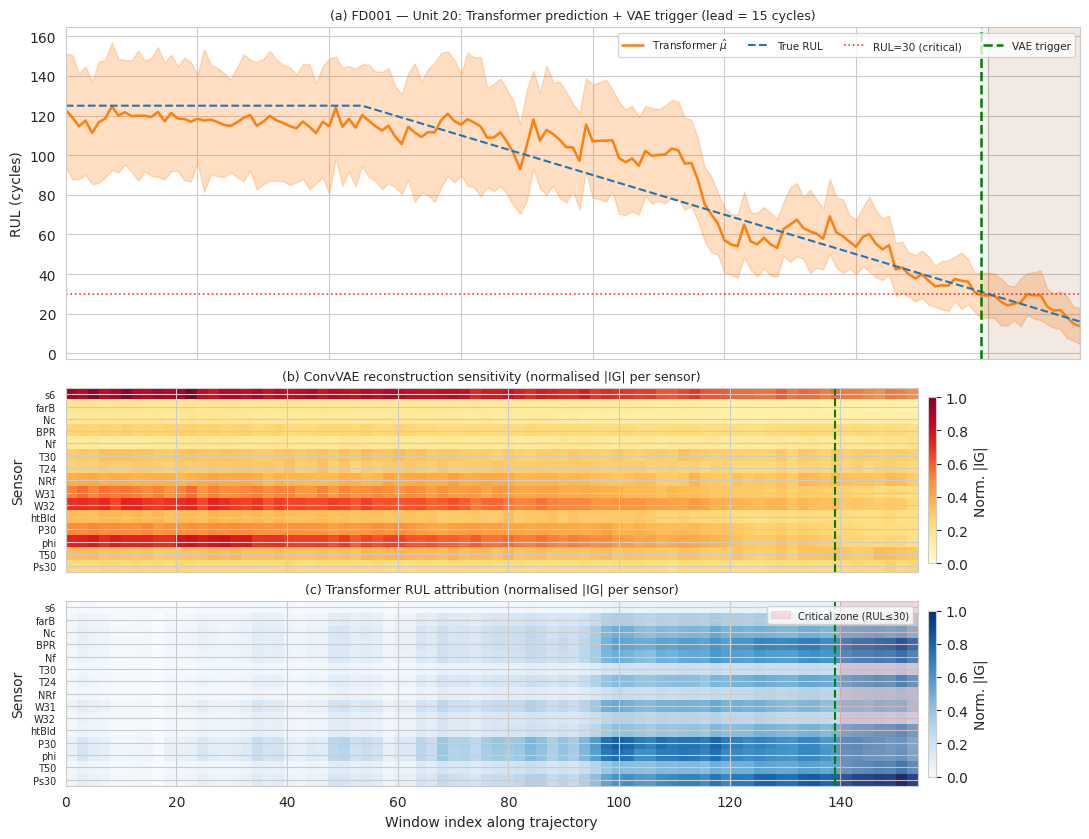
\includegraphics[width=\linewidth]{figures/attribution_fd001.pdf}%
}{%
  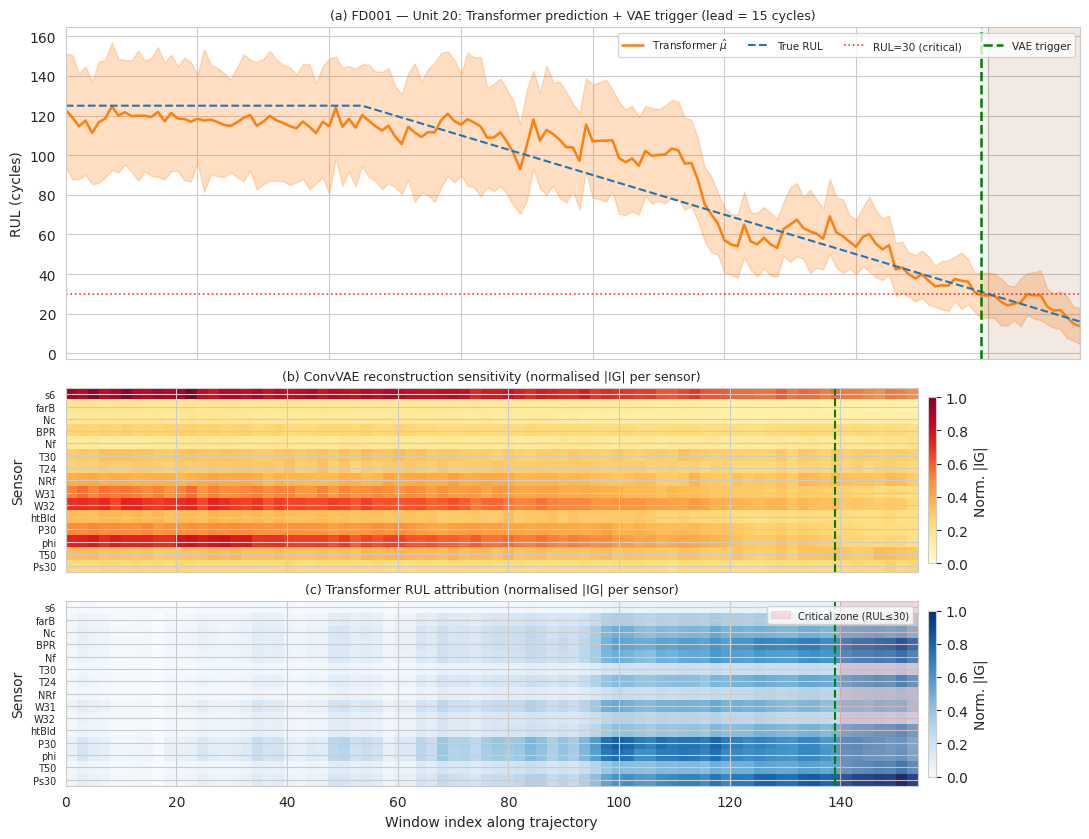
\includegraphics[width=\linewidth]{figures/attribution_fd001.png}%
}
\caption{Atribución por Gradientes Integrados para la unidad 20 de FD001 ($\tau{=}P_{99}$, persistencia $p{=}3$). (a)~Predicción del Transformer ($\hat\mu \pm 2\hat\sigma$ MC Dropout) frente al RUL verdadero; línea de puntos verde: disparo del VAE; sombreado rojo: zona crítica (RUL\,$\le$\,30). (b)~$|\mathrm{GI}|$ normalizado para el error de reconstrucción del ConvVAE: los sensores de temperatura y presión (T50, Ps30, P30) impulsan la señal de anomalía. (c)~$|\mathrm{GI}|$ normalizado para la predicción de RUL del Transformer: la atribución se concentra en T50 y Ps30 en la zona crítica, consistente con el patrón de sensibilidad del ConvVAE en el panel~(b).}
\label{fig:attribution}
\end{figure}

%% =====================================================================
\section{Conclusiones y trabajo futuro}\label{sec:conclusions}

Hemos propuesto un sistema jerárquico de anomalías a RUL que combina un autoencoder variacional convolucional unidimensional, una métrica de zona crítica (RMSE@crítico) y una capa de compuerta cuantificada con métricas a nivel de sistema (tiempo de adelanto, TPR\textsubscript{sys}, FAR\textsubscript{sys}). Evaluado en los cuatro subconjuntos de datos C-MAPSS con $N_{\mathrm{semillas}}{=}10$ ejecuciones deterministas, ICs bootstrap al 95\,\% y pruebas de Wilcoxon pareadas, el sistema proporciona 33--56\,ciclos de tiempo de adelanto medio con un TPR en zona crítica del 80--100\,\%, y un RMSE absoluto en zona crítica de 5{,}4--10{,}1\,ciclos. En los dos conjuntos de datos multi-régimen (FD002, FD004) el mejor regresor por conjunto de datos orquestado por la compuerta (Transformer y CNN+LSTM respectivamente) iguala o mejora el RMSE publicado de la última ventana de prueba; esto refleja la fortaleza de los regresores individuales más que de la capa de compuerta, cuya contribución es la señal operacional cuantificada (tiempo de adelanto, $\mathrm{TPR}_{\mathrm{sys}}$, $\mathrm{FAR}_{\mathrm{sys}}$) y no el RMSE bruto.

\subsection{Limitaciones}\label{sec:limitations}

Deben discutirse abiertamente dos limitaciones.

(i)~La FAR a nivel de sistema es del 17--23\,\% en los conjuntos de datos multi-régimen. Esto es aceptable para un despliegue de alarma con confirmación pero elevado para decisiones totalmente automatizadas. Un VAE condicional al régimen (un umbral por régimen) es la vía más probable para reducirlo.

(ii)~La cobertura MC Dropout bruta se degrada en FD002 y FD004 (PICP\,$\le$\,75\,\%, ECE\,$\ge$\,0{,}11). Esto se aborda mediante el escalado post-hoc de $\hat\sigma$ de la Sección~\ref{sec:results-mc}, que restaura el PICP al 90--95\,\% y reduce el ECE por debajo de 0{,}07 (Tabla~\ref{tab:recal}); una recalibración por régimen que evite el compromiso de factor único en datos multi-régimen queda para trabajo futuro.

\subsection{Trabajo futuro}\label{sec:futurework}

\begin{sloppypar}
Cuatro direcciones se desprenden naturalmente de los presentes resultados: (i)~VAEs condicionales al régimen para reducir $\mathrm{FAR}_{\mathrm{sys}}$ en conjuntos de datos multi-régimen; (ii)~recalibración post-hoc del MC Dropout; (iii)~ensamblados CNN+LSTM\,$\oplus$\,Transformer ponderados por conjunto de datos, motivados por la complementariedad Wilcoxon de la Sección~\ref{sec:results-rul}; (iv)~mapas de atribución \emph{condicionales al régimen} que, construyendo sobre el análisis de Gradientes Integrados por conjunto de datos ya reportado en la Sección~\ref{sec:results-attribution}, expondrían si diferentes puntos de operación activan diferentes sensores de degradación, un hallazgo directamente relevante para la aceptación regulatoria bajo la hoja de ruta de IA de la EASA~\citep{easa2025roadmap}. Una quinta dirección a más largo plazo es la integración de grandes modelos de series temporales preentrenados adaptados mediante ajuste de bajo rango, un enfoque emergente ya explorado en C-MAPSS~\citep{chakravarty2025llm4ts}, que nuestra capa de compuerta podría orquestar como regresor de alta fidelidad cuando se dispara. Finalmente, una variante exploratoria de DeepSurv basada en Cox evaluada durante el desarrollo no produjo un ranking de supervivencia útil a partir de características de la última ventana; su rediseño con un estimador de Breslow y representaciones multi-ventana es una dirección complementaria hacia la estimación probabilística del tiempo hasta el fallo.
\end{sloppypar}

%% =====================================================================
\clearpage
\section*{Declaración de contribución de autoría CRediT}

\textbf{Rafael Pecino Bonilla}: Conceptualización, Metodología, Software, Validación, Análisis formal, Investigación, Curación de datos, Escritura -- borrador original, Visualización. \textbf{Jesús Gil}: Conceptualización, Supervisión, Escritura -- revisión y edición.

\section*{Declaración de intereses en competencia}

Los autores declaran que no tienen intereses financieros en competencia conocidos ni relaciones personales que puedan haber influido en el trabajo reportado en este artículo.

\section*{Disponibilidad de datos y código}

El conjunto de datos C-MAPSS está disponible públicamente en el Repositorio de Datos de Pronóstico de la NASA~\citep{saxena2008damage}. El código fuente del pipeline, las semillas deterministas, los registros de ejecución y los hashes SHA-256 utilizados para producir cada tabla y figura de este artículo se publican en el repositorio del proyecto \url{https://github.com/rafapecino/TFM-AeroEngine-Anomaly-RUL-VAE-TFT} (SHA-256 del registro de ejecución: \texttt{662200fc9747}). Las convenciones sobre la construcción de ventanas deslizantes, la agrupación de regímenes y el etiquetado de RUL por tramos fueron verificadas cruzadamente con líneas base de la comunidad de código abierto~\citep{panara_cmapss_repo,mohyunho_ncmapss_repo} para garantizar que los números reportados siguen el protocolo canónico de C-MAPSS y permanecen comparables con el estado del arte.

\section*{Agradecimientos}

Los autores agradecen al Máster Universitario en Inteligencia Artificial (MUIA) de la Universidad Alfonso X El Sabio (UAX, Madrid, España) el entorno académico en el que se desarrolló este trabajo.

%% =====================================================================
\bibliographystyle{elsarticle-harv}
\bibliography{references}

\end{document}
